\documentclass[11pt]{scrartcl}
\usepackage[T1]{fontenc}
\usepackage[a4paper, left=3cm, right=2cm, top=2cm, bottom=2cm]{geometry}
\usepackage[activate]{pdfcprot}
\usepackage[ngerman]{babel}
\usepackage[parfill]{parskip}
\usepackage[utf8]{inputenc}
\usepackage{kurier}
\usepackage{amsmath}
\usepackage{amssymb}
\usepackage{xcolor}
\usepackage{epstopdf}
\usepackage{txfonts}
\usepackage{fancyhdr}
\usepackage{graphicx}
\usepackage{prettyref}
\usepackage{hyperref}
\usepackage{eurosym}
\usepackage{setspace}
\usepackage{units}
\usepackage{eso-pic,graphicx}
\usepackage{icomma}
\usepackage{pdfpages}

\definecolor{darkblue}{rgb}{0,0,.5}
\hypersetup{pdftex=true, colorlinks=true, breaklinks=false, linkcolor=black, menucolor=black, pagecolor=black, urlcolor=darkblue}



\setlength{\columnsep}{2cm}


\newcommand{\arcsinh}{\mathrm{arcsinh}}
\newcommand{\asinh}{\mathrm{arcsinh}}
\newcommand{\ergebnis}{\textcolor{red}{\mathrm{Ergebnis}}}
\newcommand{\fehlt}{\textcolor{red}{Hier fehlen noch Inhalte.}}
\newcommand{\betanotice}{\textcolor{red}{Diese Aufgaben sind noch nicht in der Übung kontrolliert worden. Es sind lediglich meine Überlegungen und Lösungsansätze zu den Aufgaben. Es können Fehler enthalten sein!!! Das Dokument wird fortwährend aktualisiert und erst wenn das \textcolor{black}{beta} aus dem Dateinamen verschwindet ist es endgültig.}}
\newcommand{\half}{\frac{1}{2}}
\renewcommand{\d}{\, \mathrm d}
\newcommand{\punkte}{\textcolor{white}{xxxxx}}
\newcommand{\p}{\, \partial}
\newcommand{\dd}[1]{\item[#1] \hfill \\}

\renewcommand{\familydefault}{\sfdefault}
\renewcommand\thesection{}
\renewcommand\thesubsection{}
\renewcommand\thesubsubsection{}


\newcommand{\themodul}{Halbleiter und Nanotechnologie}
\newcommand{\thetutor}{Prof. Förster}
\newcommand{\theuebung}{Übung 3}

\pagestyle{fancy}
\fancyhead[L]{\footnotesize{C. Hansen}}
\chead{\thepage}
\rhead{}
\lfoot{}
\cfoot{}
\rfoot{}

\title{\themodul{}, \theuebung{}, \thetutor}


\author{Christoph Hansen \\ {\small \href{mailto:chris@university-material.de}{chris@university-material.de}} }

\date{}


\begin{document}

\maketitle

Dieser Text ist unter dieser \href{http://creativecommons.org/licenses/by-nc-sa/4.0/}{Creative Commons} Lizenz veröffentlicht.

\textcolor{red}{Ich erhebe keinen Anspruch auf Vollständigkeit oder Richtigkeit. Falls ihr Fehler findet oder etwas fehlt, dann meldet euch bitte über den Emailkontakt.}

\tableofcontents


\newpage



\section{Aufgabe 1}

\subsection*{a)}

\begin{align*}
P_1 V &= \nu R T_1 \\
P_2 V &= \nu R T_2 \\
\intertext{Wir setzen ein:}
T_2 &= \frac{P_2 V}{\nu R} = \frac{P_2 T}{P_1} = \frac{P_2}{P_1} \cdot T_1
\intertext{Wenn nun bei $T_1$ der Druck bekannt ist, dann kann man $P_2$ messen und die Temperatur $T_2$ berechnen. $P_2$ wird gemessen über:}
P_2 &= P_1 + \rho_{Hg} \cdot g \cdot \Delta h
\end{align*}


\subsection*{b)}

Wir setzen die Werte in SI Einheiten ein:

\begin{align*}
P_2 &= 10^5 + 13645 \cdot 9,81 \cdot 0,08 = \unit[1,107 \cdot 10^5]{Pa}
\intertext{Die Temperatur ist dann:}
T_2 &= \frac{1,107 \cdot 10^5}{10^5} \cdot 300 = \unit[332]{K}
\end{align*}


\section{Aufgabe 2}

Wir stellen zunächst drei Gleichungen auf, die wir dann ineinander einsetzen können, daraus erhalten wir dann die gewünschte Formel:

\begin{align*}
&\text{I)}  & P_T V &= \nu R T = \nu R \left( 273,15 \cdot \theta \right) \\
&\text{II)}  & P_{100} V &= \nu R T_{100} = \nu R \left( 273,15 + 100 \right) \\
&\text{III)}  & P_0 V &= \nu R T_0 = \nu R \left( 273,15 \right)
\end{align*}
Nun ziehen wir III von II ab:
\begin{align*}
\left( P_{100} - P_0 \right) V &= \nu R \cdot 100 \\
\Leftrightarrow \nu R &= \frac{P_{100} - P_0}{100} \cdot V
\intertext{Wir ziehen nun I von II ab:}
\nu R \theta &= \left( P_T - P_0 \right) \cdot V \\
\Leftrightarrow \frac{P_{100} - P_0}{100} \cdot V \theta &= \left( P_T - P_0 \right) \cdot V \\
\Leftrightarrow \theta &= \frac{P_T - P_0}{P_{100} - P_0} \cdot 100
\end{align*}


\section{Aufgabe 3}

Wir müssen in beiden Aufgabenteilen einfach nur in die ideale Gasgleichung einsetzen.

\subsection*{a)}

\begin{align*}
PV = \nu RT \Leftrightarrow V &= \frac{RT}{P} = \frac{8,3145 \cdot 273,15}{1,013 \cdot 10^5} = \unit[22,4]{l}  
\end{align*}


\subsection*{b)}

\begin{align*}
PV = \nu RT \Leftrightarrow V &= \frac{RT}{P} = \frac{8,3145 \cdot 298,15}{1,013 \cdot 10^5} = \unit[24,79]{l}  
\end{align*}


\section{Aufgabe 4}

Wir nehmen an, das Raumtemperatur $\unit[300]{K}$ und $\unit[1]{atm} = \unit[9,811 \cdot 10^4]{Pa}$:

\subsection*{a)}

Wir berechnen zunächst die molare Masse von $CO_2$:

\begin{align*}
M(CO_2) &= \unit[12]{g} + 2 \cdot \unit[16]{g} = \unit[44]{g}
\intertext{Damit erhalten wir unser $\nu$:}
\nu &= \frac{100}{44} = \unit[2,27]{mol/l}
\intertext{Nun können wir wieder in die ideale Gasgleichung einsetzen:}
V = \frac{\nu RT}{P} &= \frac{2,27 \cdot 8,134 \cdot 300}{9,811 \cdot 10^4} = \unit[57,8]{l}
\end{align*}


\subsection*{b)}

\begin{align*}
P &= \frac{\nu RT}{V} &= \frac{2,27 \cdot 8,134 \cdot 300}{80 \cdot 10^{-3}} = \unit[7,071 \cdot 10^4]{Pa}
\end{align*}


\section{Aufgabe 5}

\subsection*{a)}

Wir lesen die Drücke aus dem Diagramm ab:

\begin{align*}
P_{294} &= \unit[64,7]{bar} \\
P_{284} &= \unit[55,9]{bar}
\end{align*}


\subsection*{b)}


Wir lesen zwei markante Punkte ab und bauen daraus den Graphen:

\begin{align*}
P_{304} &= \unit[73,4]{bar} \\
P_{274} &= \unit[48,2]{bar}
\end{align*}

Der Graph sollte in etwa linear sein mit der Temperatur auf der x-Achse und einer Steigung von $\frac{\Delta P}{\Delta T} = \unit[0,786]{bar/K}$



\subsection*{c)}

Wir müssen uns zunächst klarmachen was $\Delta V$ ist. $\Delta V$ ist die Volumendifferenz zwischen dem gasigen und dem flüssigen Zustand, also gilt $\Delta V = V_g - V_f$. Nun lösen wir nach der Entalpie auf:

\begin{align*}
\Delta H &= \frac{\p P}{\p T} \cdot \Delta V \cdot T
\intertext{Nun bestimmen wir die $\Delta V$ bei den angegebenen Temperaturen:}
\Delta V(\unit[274]{K}) &= \unit[2,22 \cdot 10^{-4}]{m^3/mol} \\
\Delta V(\unit[284]{K}) &= \unit[1,601 \cdot 10^{-4}]{m^3/mol} \\
\Delta V(\unit[294]{K}) &= \unit[1,1 \cdot 10^{-4}]{m^3/mol} 
\intertext{Nun berechnen wir die Enthalpie:}
\Delta H_{\unit[274]{K}} &= 0,786 \cdot 10^5 \cdot 2,22 \cdot 10^{-4} \cdot 274 = \unit[4,78 \cdot 10^3]{J/mol} \\
\Delta H_{\unit[284]{K}} &= 0,786 \cdot 10^5 \cdot 2,22 \cdot 10^{-4} \cdot 284 = \unit[3,57 \cdot 10^3]{J/mol} \\
\Delta H_{\unit[294]{K}} &= 0,786 \cdot 10^5 \cdot 2,22 \cdot 10^{-4} \cdot 294 = \unit[2,31 \cdot 10^3]{J/mol} \\
\end{align*}


\subsection*{d)}

Mit der Annahme $V_g >> V_f$ vereinfacht sich die Gleichung aus dem vorigen Aufgabenteil zu:

\begin{align*}
\frac{\p P}{\p T} &= \frac{\Delta H}{T V_g} 
\intertext{Nutze $PV = RT$:}
\Leftrightarrow \frac{\p P}{\p T} &= \frac{\Delta H \cdot P}{T^2 R}
\intertext{Teile die Integration auf zwei Seiten auf:}
\frac{\p P}{P} &= \frac{\Delta H \p T}{T^2 R} 
\intertext{Wir führen folgende Integration aus $\int_{P_1}^{P_2}$ und $\int_{T_1}^{T_2}$ und erhalten:}
\ln(P_2) - \ln(P_1) &= - \frac{\Delta H}{R} \left( \frac{1}{T_2} - \frac{1}{T_1} \right) \\
\Leftrightarrow \frac{\p \ln(P)}{\p \frac{1}{T}} &= - \frac{\Delta H}{R}
\end{align*}

\begin{figure}[h]
	\centering
	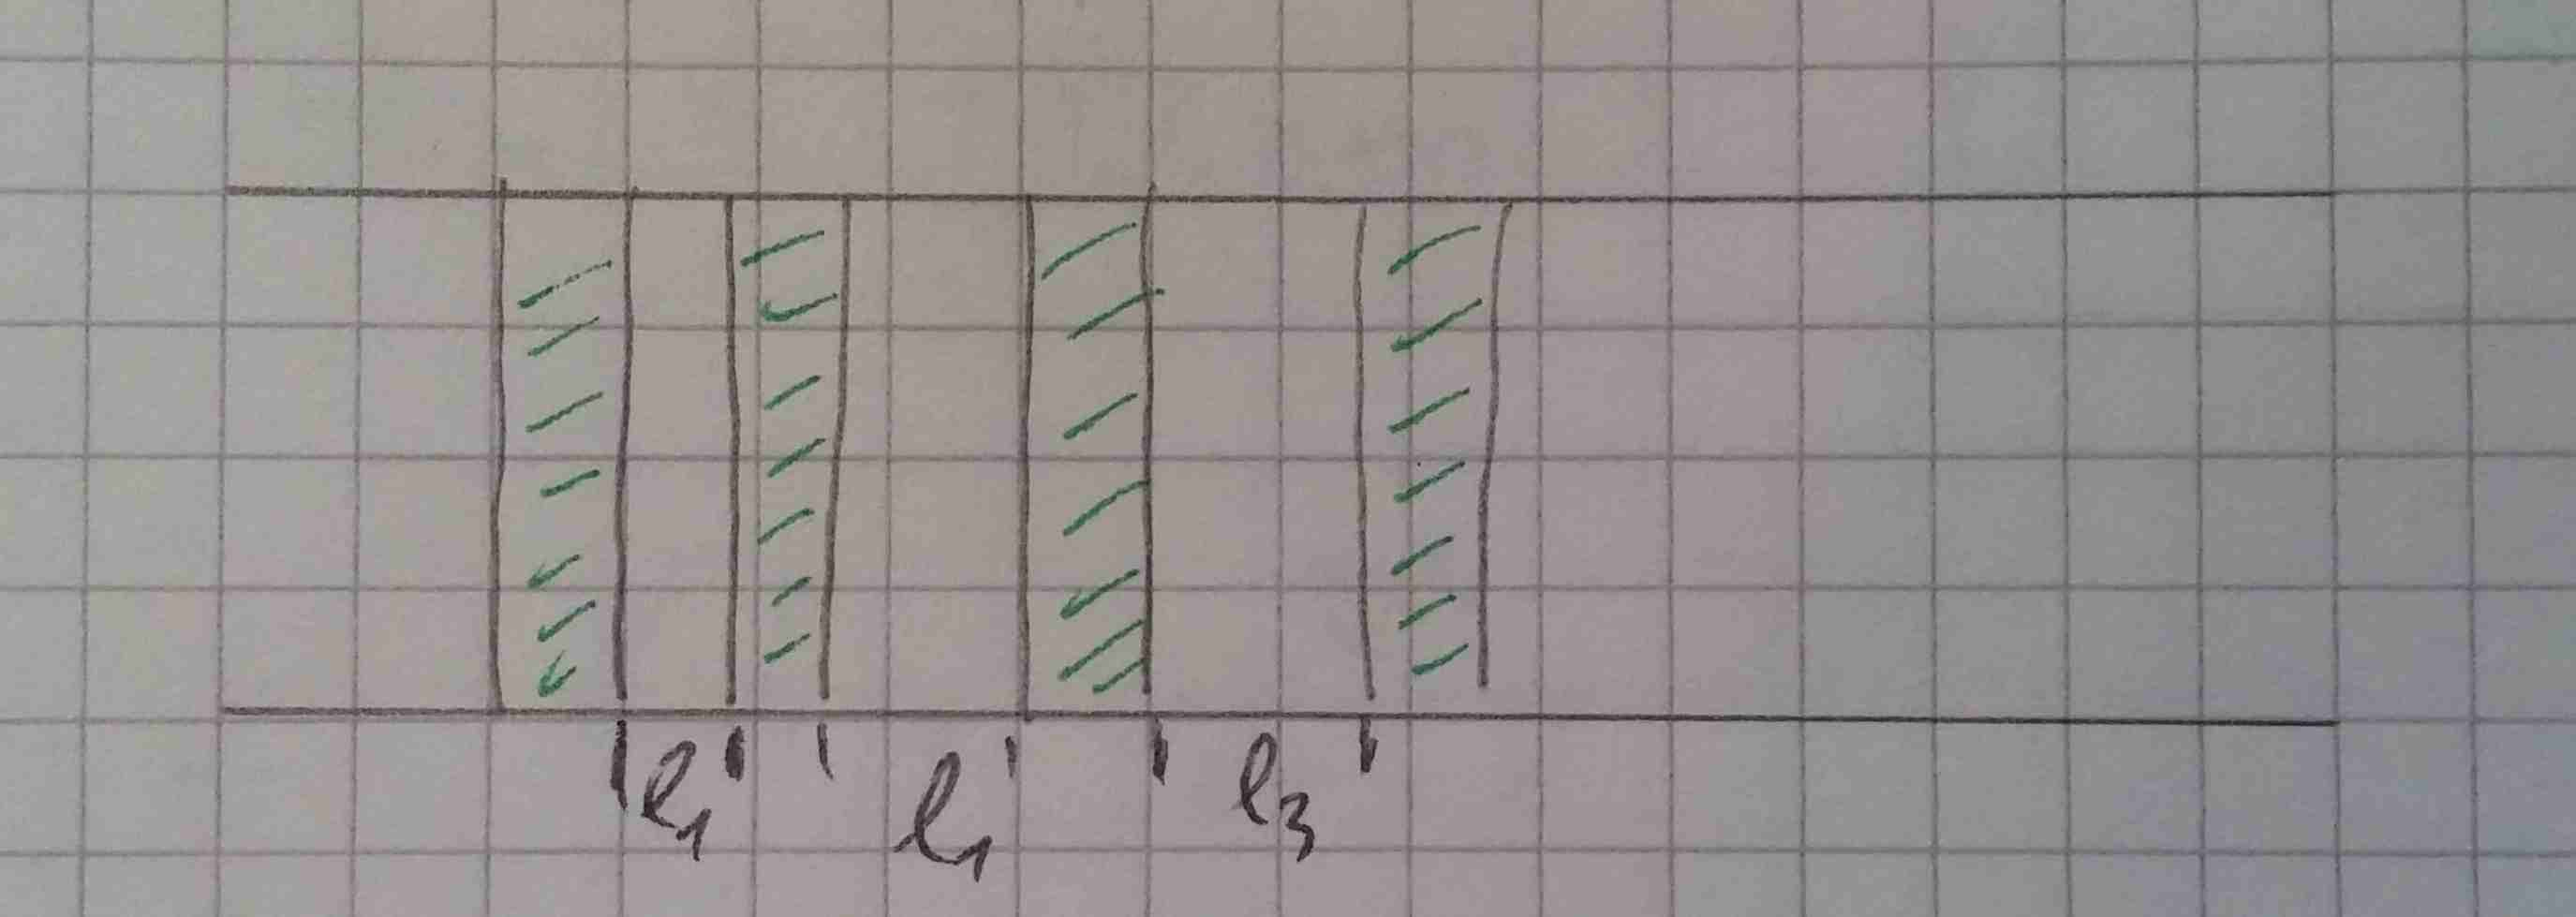
\includegraphics[scale=0.15]{A5_1.jpg}
	\caption{$\frac{\Delta \ln(P)}{\Delta \frac{1}{T}} = - \frac{\Delta H}{R}$}
\end{figure}


\newpage

\subsection*{e)}

Wir bauen uns zuerst eine Tabelle mit ein paar Eckdaten, die wir schon kennen:

\hfil \\

\begin{center}
	\begin{tabular}{|c|c|c|c|}
		$T$ & $P_D$ & $\ln(P_D)$ & $\frac{1}{T}$ \\ 
		\hline
		$274$ & $48,2 \cdot 10^5$ & $15,39$ & $3,65 \cdot 10^{-3}$ \\ 
		$284$ & $55,9 \cdot 10^5$ & $15,54$ & $3,52 \cdot 10^{-3}$ \\ 
		$294$ & $64,7 \cdot 10^5$ & $15,68$ & $3,4 \cdot 10^{-3}$ \\ 
	\end{tabular} 
\end{center}

\hfil \\

Man erhält dann diesen Graphen:

\begin{figure}[h]
	\centering
	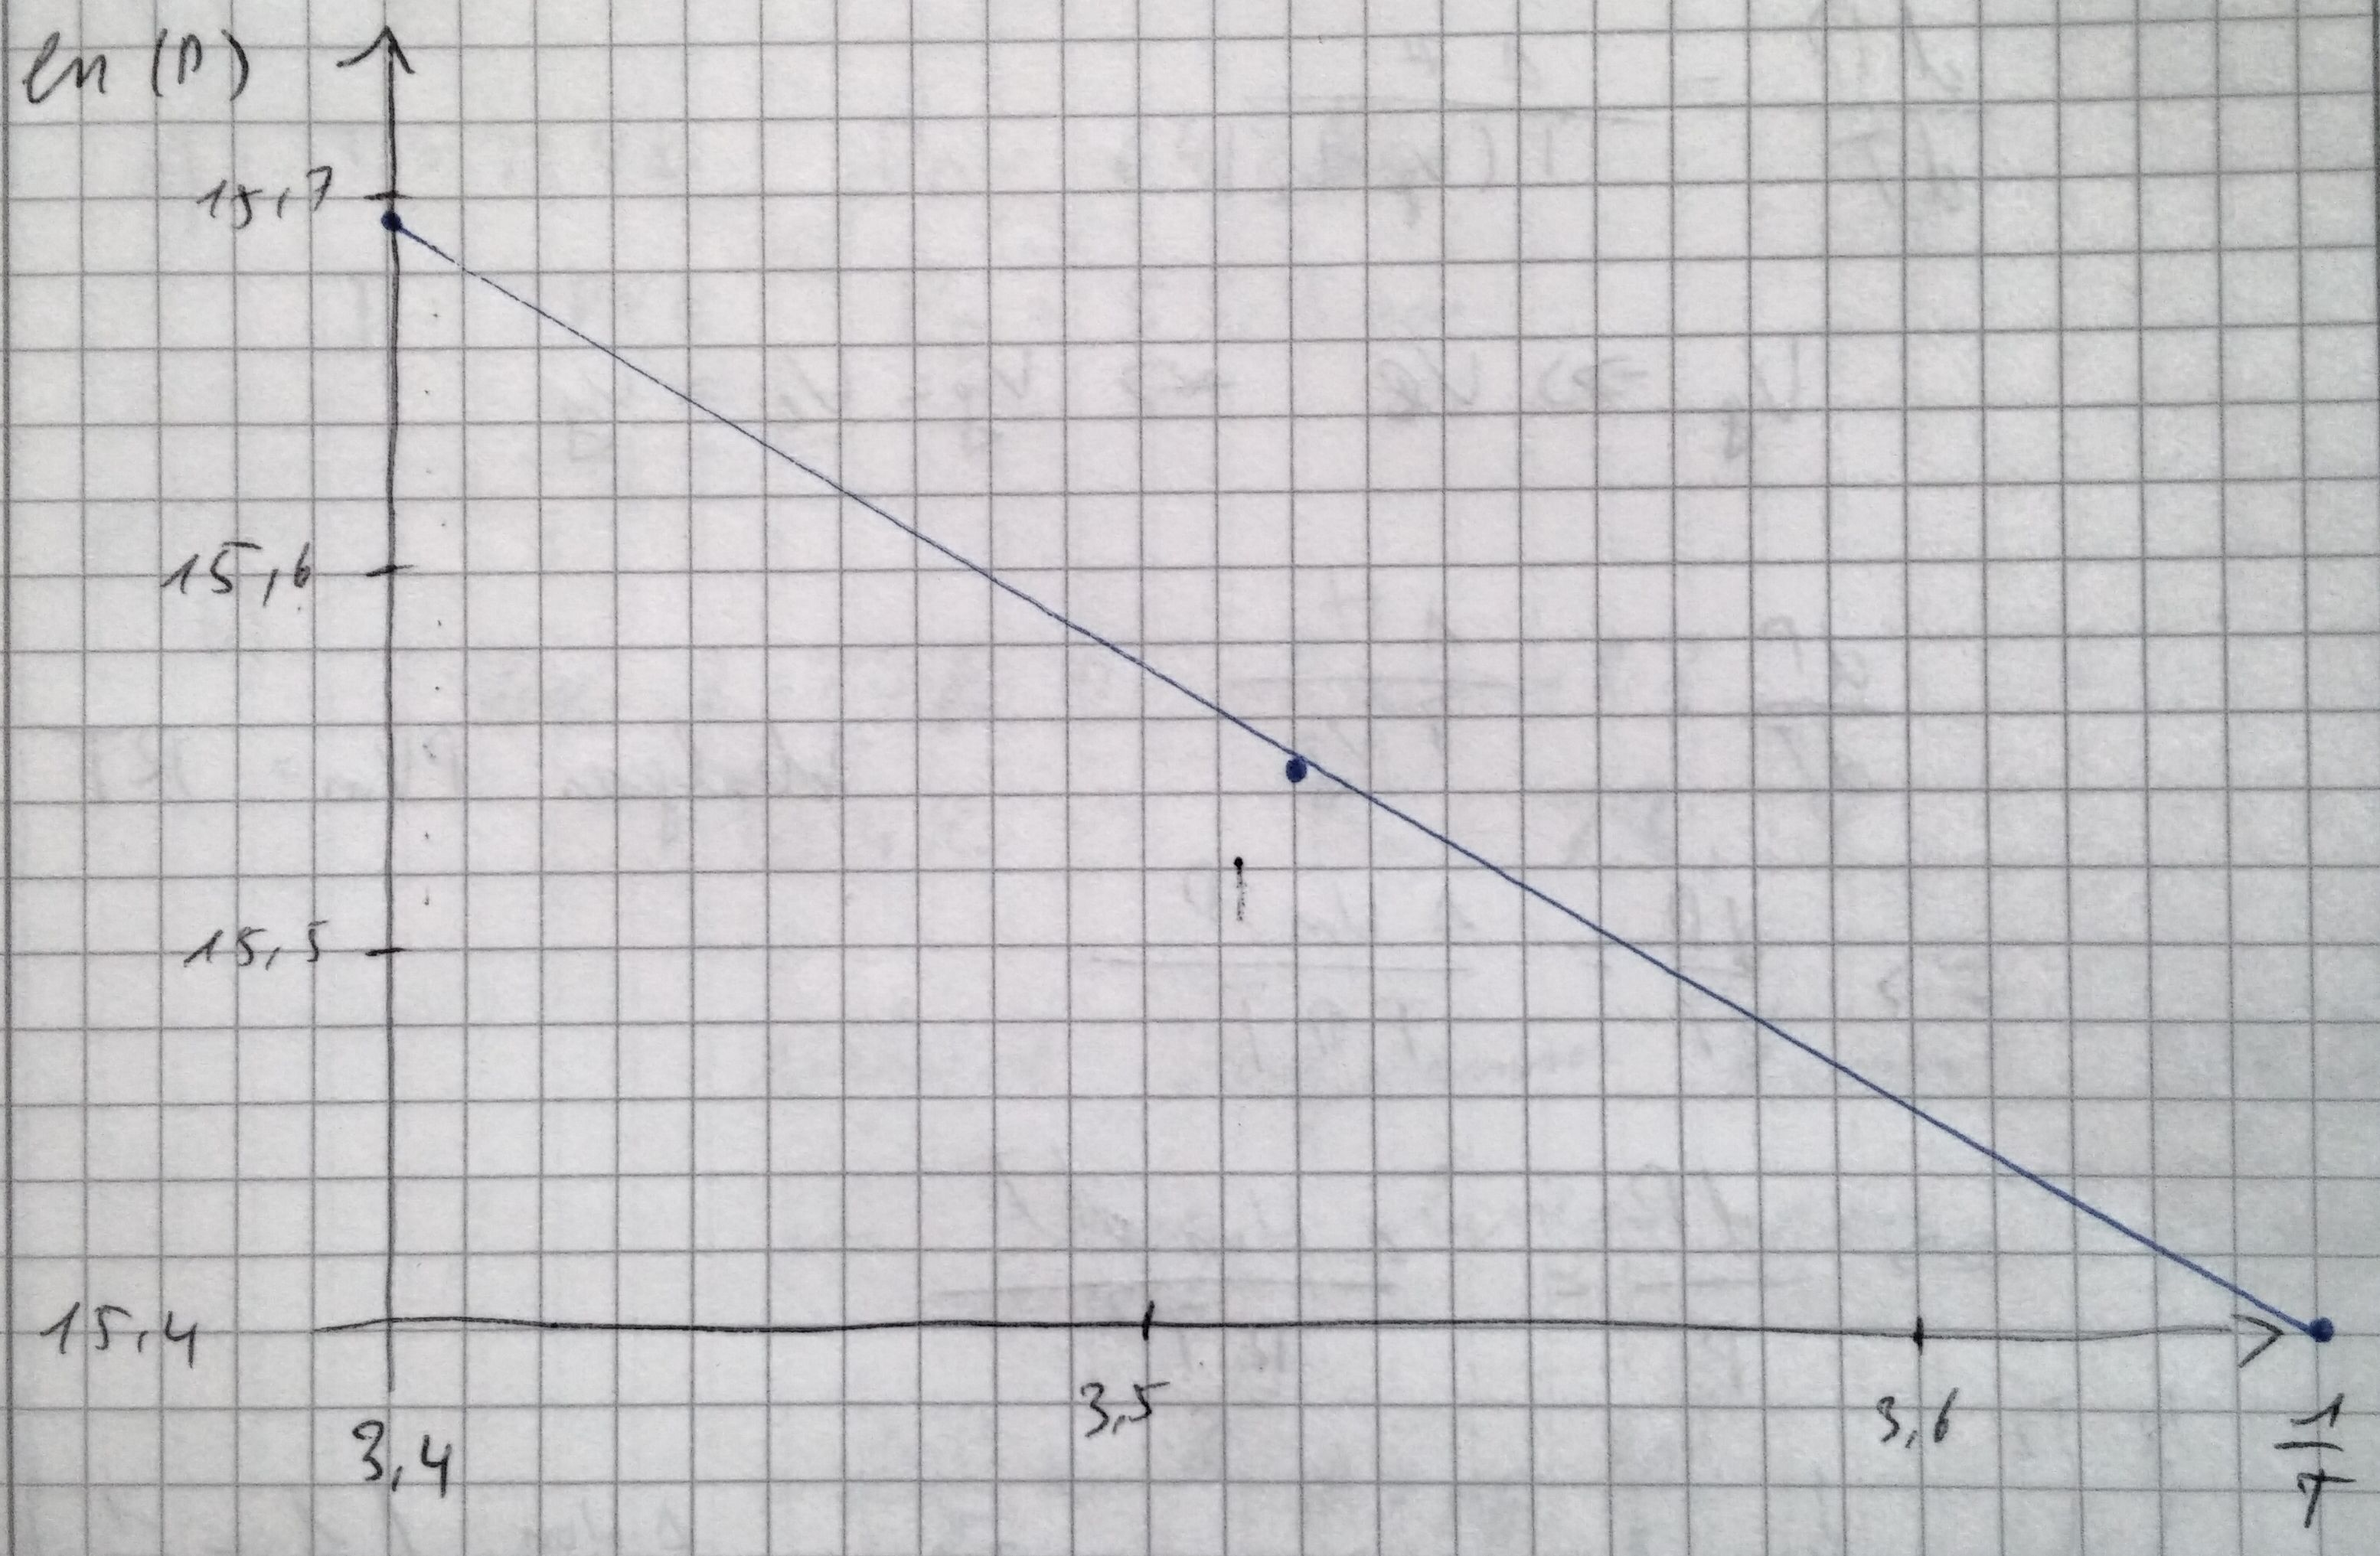
\includegraphics[scale=0.15]{A5_2.jpg}
	\caption{$\frac{\Delta \ln(P)}{\Delta \frac{1}{T}} = -1,16 \cdot 10^{-3}$}
\end{figure}

\begin{align*}
\Delta H = R \cdot 1,16 \cdot 10^{3} = \unit[9,64]{kJ/mol} = \unit[219]{kJ/kg}
\end{align*}


\newpage


\subsection*{f)}

\begin{figure}[h]
	\centering
	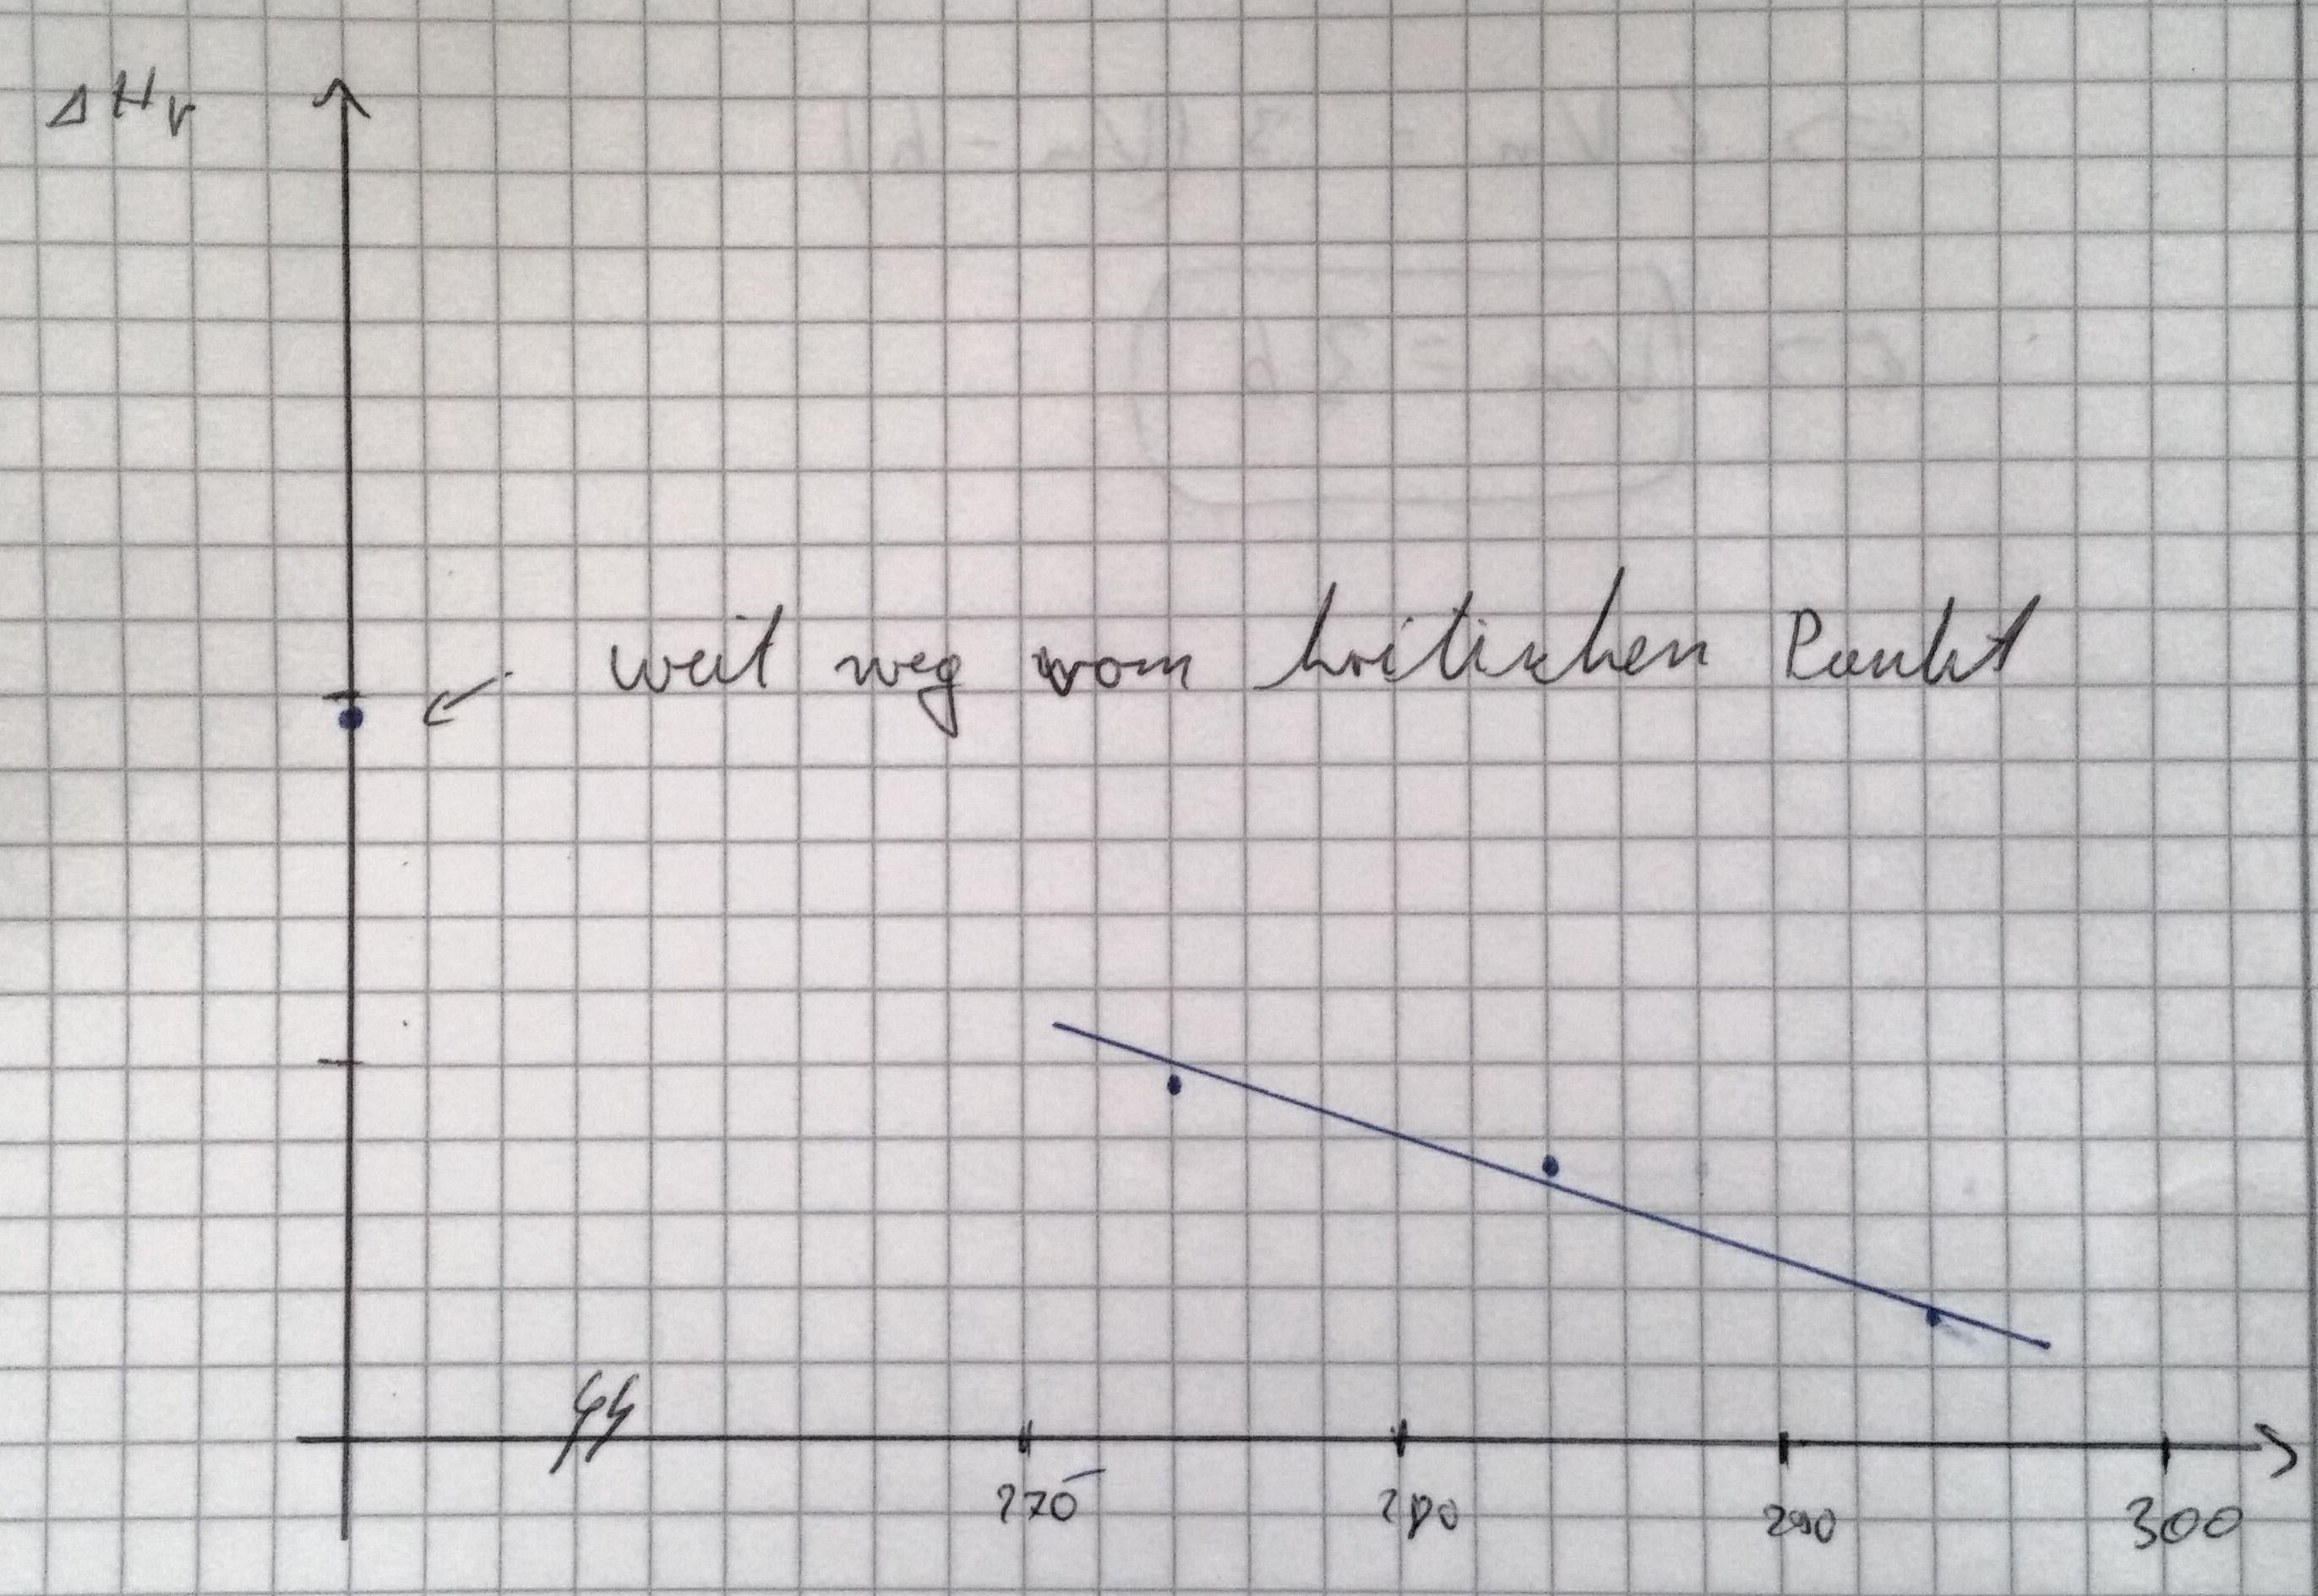
\includegraphics[scale=0.15]{A5_3.jpg}
	\caption{}
\end{figure}














\end{document}